\documentclass{pgnotes}

\title{Cloud Computing Introduction}

\begin{document}

\maketitle

\section{What's it all about?}
\label{sec:whats-it-all-about}

Cloud computing is essentially renting computing resources as needed to build-up systems in a quick self-service way.
Think of it as booking a ryanair flight (vs buying your own plane), renting a car in a foreign country (vs buying one) or taking an AirBNB (vs buying a holiday home).
Like travel planning, learning how to design, provision and utilise cloud computing resources is a learned skill developed through practice.

\section{Backend}
\label{sec:backend}

In this module we will primarily focus on backend processing, as opposed to frontend computing (desktops, mobile devices).
As with any computing system, backend processing generally involves three key ingredients:
\begin{description}
\item[Compute power:] in the form of CPU cycles in server hardware, possibly shared by a hypervisor and managed by an operating system.
\item[Storage:] in the form of magentic disks, SSDs, tape and other media that is directly attached to server hardware or connected over a network. 
\item[Connectivity:] so that the remote computing resource can be utilised by its intended consumers.
\end{description}

The earliest large computers (so-called mainframes like IBM System/360) led to smaller minicomputers (DEC PDP 8/11, VAX, IBM AS/400) and later on to PC-based servers running Linux / UNIX / Windows.
Yet many of the ideas we'll see in Cloud particular around pricing and pay-per-use actually were and are evident in Mainframes. 

\subsection{Batch processing}
\label{sec:batch-processing}

Historically a lot of backend processing was batch-oriented.
This is still encountered in business processes (e.g. a bank processes payments overnight or utility sends a bill once a month).

\subsection{Services}
\label{sec:services}

The alternative to batch processing is service-based processing, where a server allows one or more clients to connect and processes data in real time. 
Services commonly encountered include:
\begin{itemize}
\item \textbf{On the public internet} are web servers (HTTP, HTTPS), file transfer protocol (FTP), domain name servers (DNS), remote shell login (SSH), remote desktop (RDP), network time protocol (NTP), remote sync (rsync), virtual private network (VPN). 
\item \textbf{Within private networks:} all of the above plus file sharing (NFS, CIFS/SMB, AFS), database servers (MySQL, PostgreSQL, Oracle etc), message brokers (ActiveMQ, RabbitMQ), media sharing (UPnP/DLNA), block storage (iSCSI), mainframe access (3270, 5250 emulation), insecure remote shell login (telnet, rsh) and custom servers.
  Many of these services in theory could run over the internet but for security, performance and other reasons they generally don't.
\end{itemize}
  
We will assume in this module that all services communicate over standard TCP/IP. 
For a given service, the client and server implement a common protocol that normally has an associated standard port number, \autoref{fig:port-numbers}

\begin{figure}[htbp]
  \centering
  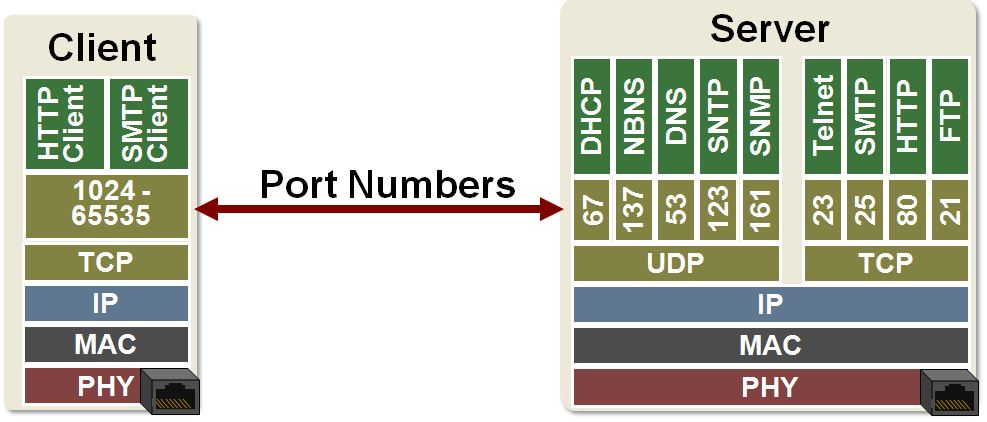
\includegraphics[width=0.5\linewidth]{port_numbers}
  \caption{Port numbers}
  \label{fig:port-numbers}
\end{figure}

\subsection{Building systems}
\label{sec:building-systems}

It is important to remember in practice that a service may be a client of another service, and that most systems of even modest complexity involve multiple interdependent services:
\begin{itemize}
\item A web application (PHP on Apache/mod\_php or Spring with Tomcat) might access a database (Oracle), a messaging queue (ActiveMQ) and an in-memory cache (Redis).
\item A file server running Windows Server provides SMB/CIFS file shares that are on a drive provisioned on an iSCSI volume shared from a FreeBSD UNIX machine. 
\end{itemize}

\section{Service requirements}
\label{sec:service-models}

Assuming we are dealing with backend server environments, our services are assumed to consist of software running on appropriate hardware.
Server hardware requires power, connectivity and cooling in a secure and fireproof environment with appropriate channels to manage the hardware remotely.
Normally we require resiliency in the infrastructural services and connectivity so that the service remains available.
We can first distinguish among a number of common patterns for where our services are hosted: 
\begin{description}
\item[On-site] within a suitably equipped data centre environment providing power, connectivity, cooling and security with the appropriate resiliency for the required service availability.
\item[Co-located] where our hardware is located in a data centre facility that provides space, power, connectivity, cooling and security with the appropriate levels of resiliency.
\item[Hosted] where a provider provisions equipment and software that we require.
  \begin{itemize}
  \item Hosted environments tend to involve manual setup and can provide both bare-metal servers, managed physical servers and virtual servers.
  \item Hosting provider will themselves be provisioning onsite or co-lo, or may be reselling from elsewhere!
  \item Many co-lo data centres also offer hosting as a service. 
  \end{itemize}
\end{description}

All of these environments require significant upfront \textit{capital expenditure}, must be right-sized from the beginning and scaling requires significant effort.


\section{Expenditure}
\label{sec:expenditure}

Setting up and running any service requires expenditure, which can be broken down into: 
\begin{description}
\item[Capital expenditure (CAPEX):] money spent on goods/services necessary for future performance. Usually fixed / non-consumable assets. CAPEX is often made using borrowed money.
\item[Operational expenditure (OPEX):] money spent on goods/services necessary for day-to-day running of the business. Often supplies/inputs into output. Needs to be self-financing if the service/business is to survive.
\end{description}
Note that whether a particular item is CAPEX or OPEX depends on the context.
To a homeowner, a bale of concrete blocks for an extension represents CAPEX.
To the shop supplying them, they are an OPEX to buy.

\textbf{Key advantage} of cloud computing is shifting CAPEX to OPEX.


\section{Cloud definition and characteristics}
\label{sec:essential-characteristics}

The term ``cloud'' primarily appeared in its current context when AWS released their so-called Elastic Compute Cloud in 2006.
Rather than an explicit definition, NIST describes five essential characteristics for a particular service to be termed a ``cloud service'':
\begin{description}
\item[On-demand self-service] allowing consumer to provision required services without human interaction.
\item[Broad network access] allowing consumer to access provisioned services over standard network interfaces (e.g. TCP/IP over internet).
\item[Resource pooling] where provider uses a large pool of resources to serve consumers on-demand, without the consumer having any affinity to a physical resource.
\item[Rapid elasticity] to enable a consumer to vertically/horizontally scale their provisioned capacity.
\item[Measured service] where a consumer pays for provisioned/used services at a relatively granular level, subject to resource limits.
\end{description}
If a service broadly meets these, then it can be termed a cloud service.
They key differentiating factors are the self-service nature, the locatation independence, the seemingly unlimited pool of resources on the backend and the ability to control and pay for what you use on a short-term basis.

\section{Main providers}
\label{sec:main-providers}

The main cloud providers are shown in \autoref{tab:main-providers}.

\begin{table}[htbp]
  \centering
  \begin{tabular}{l l l}
    \toprule
    \textbf{Provider} & \textbf{Service} & ~ \\ 
    \midrule
    Amazon & Amazon Web Services & AWS \\
    Microsoft & Azure & ~ \\
    Google & Google Compute Cloud & \\
    IBM & IBM Cloud & \\
    Digital Ocean & & \\
    \bottomrule
  \end{tabular}
  \caption{Main providers}
  \label{tab:main-providers}
\end{table}

\section{Cloud service models}
\label{sec:cloud-service-models}

Within the cloud NIST describes three different service models:
\begin{description}
\item[Infrastructure as a Service (Iaas):] provider makes available compute power in the form of virtual machines, storage in multiple forms and allows networks to be constructed to link these resources together. Obviously you don't have access to the hardware.
  \begin{itemize}
  \item \textbf{How to identify:} you are dealing with CPU / RAM / storage specifications, operating systems (Windows / Linux), networking (IP addressing, subnet masks).
  \end{itemize}
\item[Platform as a Service (PaaS):] components such as database servers, integration components (queues, notification systems), object storage that can be provisioned directly from the web / CLI. 
  \begin{itemize}
  \item \textbf{How to identify:} you're not directly interacting with CPU, RAM, storage, OS, networking.
  \end{itemize}
\item[Software as a Service (SaaS):] provider makes software available for use over standard network protocols (HTTP/RDP/SSH) either by humans or an API (e.g. Github).  
\end{description}
In reality, the lines between IaaS, PaaS and SaaS are often blurred.
They are probably better thought of as a continuum from SaaS through PaaS to IaaS. 
It can be difficult to place many cloud services exclusively into one of these three categories, nor is it necessary to.
Many solutions built including cloud technologies will include all three.


\begin{figure}[htbp]
 \centering
 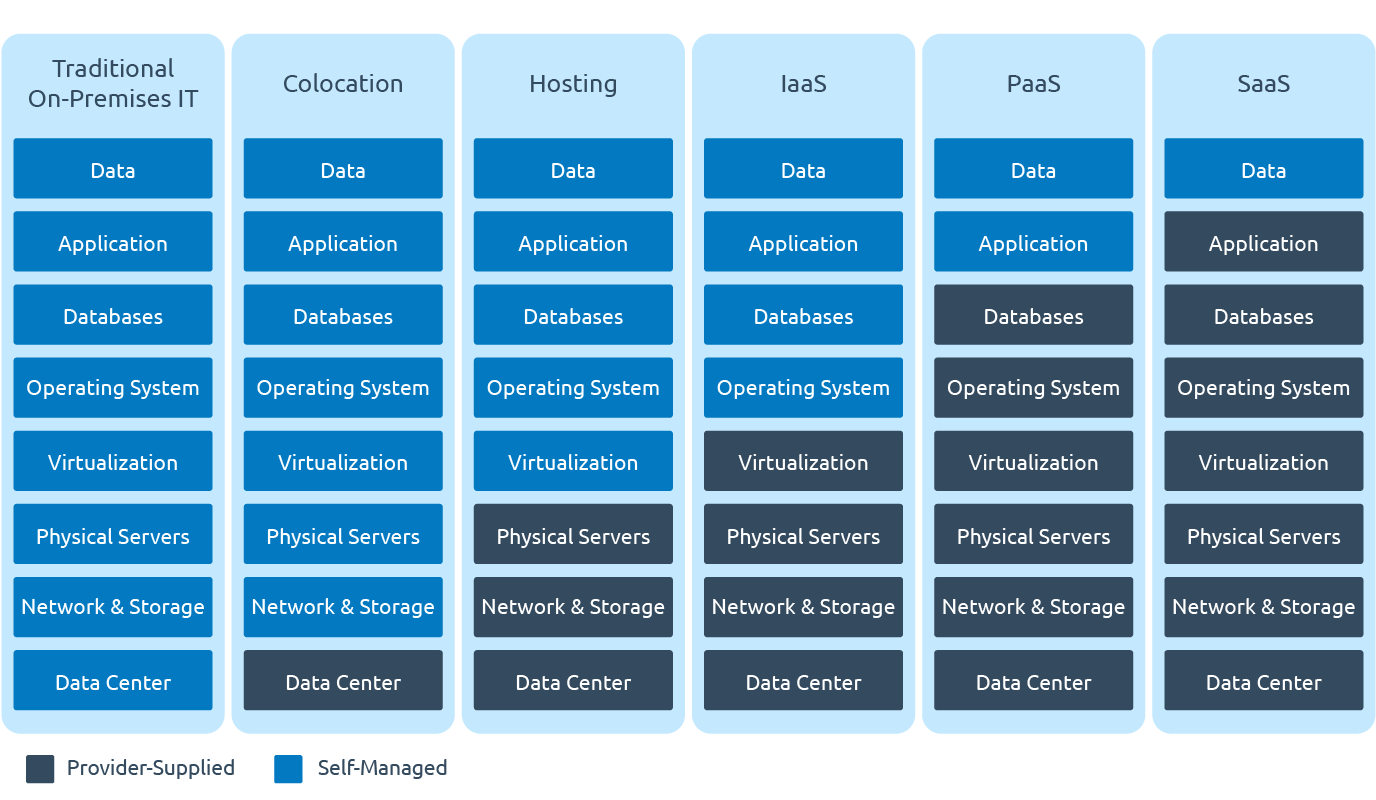
\includegraphics[width=1.0\linewidth]{cloud_service_models}
 \caption{Cloud service models}
 \label{fig:cloud-service-models}
\end{figure}

\section{Interface}
\label{sec:interface}

Most cloud providers support a number of channels for provisioning resources and interacting with them: 

\begin{description}
\item[Web console] providing manual point-and-click interaction
  \begin{itemize}
  \item Easy to explore, BUT not a good idea to use exclusively long-term.
  \end{itemize}
\item[Command-line interface (CLI)] command can be installed on your own computer and can be run from PowerShell / Bash
  \begin{itemize}
  \item It can be tempting to avoid the CLI but this is generally a foolish decision in terms of time, precision and opportunities to automate!
  \item The CLI commands for most providers (e.g. \texttt{aws}, \texttt{gcloud}) provide an extensive online help system with examples. For AWS try typing \texttt{aws help}.
  \item CLI avoids cumbersome manual login process - another reason to use it.
  \end{itemize}
\item[Software Development Kit (SDK):] for applications running on cloud and elsewhere (local desktop, mobile) that need to interact with cloud resources.
  \begin{itemize}
  \item We won't spend much time with SDKs but may encounter them later on!
  \item Example: a Python script needs to push a message to a messaging queue provisioned on AWS SQS.
  \end{itemize}
\end{description}

\section{Costs}
\label{sec:costs}

Metered costs for cloud usage depend on the particular service under discussion.
Broadly, these will break down into:

\begin{table}[htbp]
  \centering
  \begin{tabularx}{1.0\linewidth}{l l X}
    \toprule
    \textbf{Charge type} & \textbf{Common units} & \textbf{Remarks} \\
    \midrule
    Setup/teardown & Per resource unit & \\
    Time-based & Days / hours / mins / seconds & Often for IaaS components \\
    Usage-based & Requests / invocations & Often for PaaS components \\
    Data Storage & MB / GB / TB etc & Data at rest \\
    Data Transfer & MB / GB / TB etc & Inbound, outbound, internal may differ \\
    \bottomrule
  \end{tabularx}
  \caption{Cost types}
  \label{tab:cost-types}
\end{table}

\section{Geographic infrastructure groups}
\label{sec:geographic-infrastructure-groups}

The major ``full service'' cloud providers separate their infrastructure geographically.
This is done for two reasons.
Firstly it lets cloud providers separate services in different geographical regions from each other for legal and business reasons.
Secondly it facilitates redundancy in case of failures. 

\begin{description}

\item[Regions] are \textbf{designed to separate data and resources} for business and legal reasons.
  
  \begin{itemize}
  \item Regions function independently of each other.  Essentially they are different instances of the cloud provider's infrastructure.
  \item Regions usually chosen such that legal environment is similar across them: e.g. varied FOI, GDPR, HIPAA, COPPA, data siphoning regulations.
  \item Provider may introduce and update services to different regions at different times.
  \item Pricing may vary across regions for the same services.
  \item Most cloud providers identify each region with both a human readable name like ``EU (Ireland)'' and a code name like \texttt{eu-west-1}. We will in class use only the code names for the most part.
  \item \textbf{Must consider region when deploying most services!}
  \end{itemize}

\item[Non-geographic regions] are purpose-specific rather than geographical, like AWS GovCloud.
  
\item[Geography] is a region-grouping that Azure use.  AWS doesn't have a multi-region grouping concept.
  \begin{itemize}
  \item Legal environment is normally consistent across all regions in a Geography.
  \end{itemize}
  
\item[Availability zones] are a \textbf{technical construct} to tolerate failures in physical infrastructure.
  \begin{itemize}
  \item
    Each AZ normally consists of $\ge 1$ data centres, each internally redundant.
    The data centres in an AZ are connected to each other by low-latency highly-redundant network links.
  \item
    AZs are identified only by a code name derived from their region code name.
    For the \texttt{eu-west-1} region the corresponding AZs are \texttt{eu-west-1a}, \texttt{eu-west-1b} and \texttt{eu-west-1c}.
  \item Note that the AZ code \texttt{a, b, c} mappings to physical AZs \textit{are not} consistent across different AWS accounts.
    This is to balance usage across AZs.
    (Many people will just choose the \texttt{a} AZ since it appears first in the list.)
  \item \textbf{In general, we need to consider AZs when deploying IaaS services but NOT PaaS.}
  \end{itemize}  

\item[Edge locations] are an entirely parallel structure provididing access points and edge caching for users of customer applications.
  These are normally a separate set of locations to the provider's regions/AZs for customer use.

\end{description}

The providers all do a better job on constantly updating their global infrastructure maps than any lecture notes will:
\begin{itemize}
\item \textbf{AWS:} \url{https://aws.amazon.com/about-aws/global-infrastructure/}
\item \textbf{Google Cloud:} has a similar breakdown of regions and AZs to AWS. \url{https://cloud.google.com/about/locations}
\item \textbf{Azure:} \url{https://azure.microsoft.com/en-us/global-infrastructure/}
\end{itemize}

\section{Service agreement}

Cloud Providers will offer their services as part of a service agreement, which specifies a number of promises, limitations and obligations, \autoref{fig:terms}:
\begin{description}
\item[Promises] are guarantees by the cloud provider of things it will do for the customer.
\item[Limitations] limit the scope of the promises that a cloud provider makes to a customer.
\item[Obligations] specify rules that a customer must comply with when using the cloud service. 
\end{description}

\begin{figure}[htbp]
  \centering
  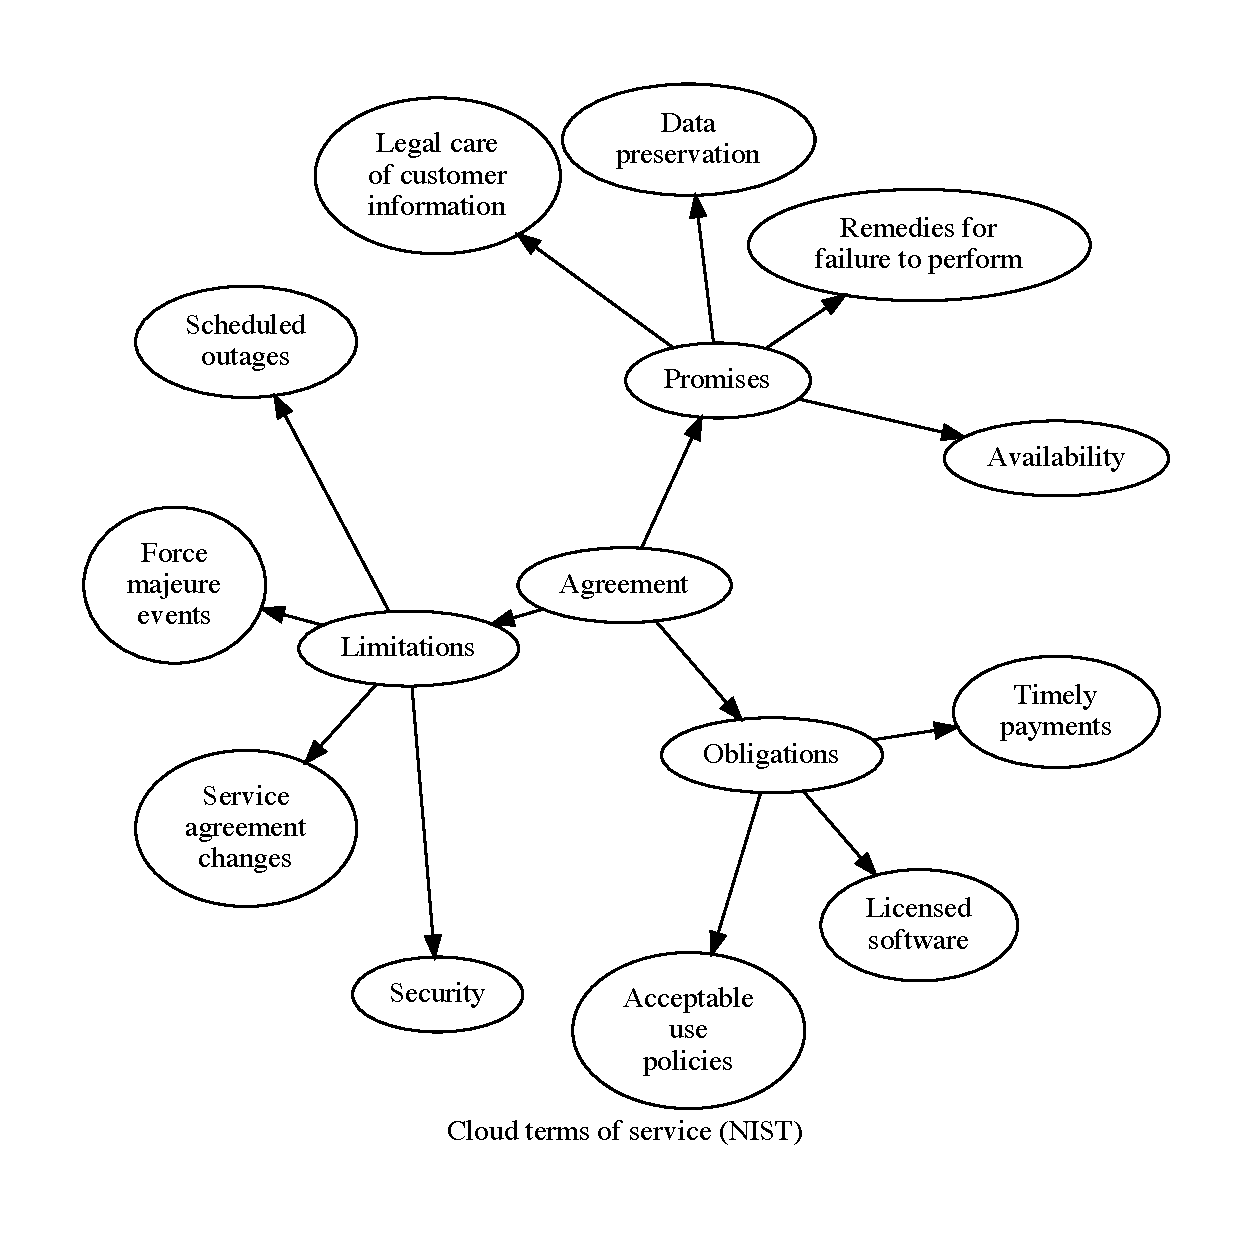
\includegraphics[width=0.75\linewidth]{terms_map}
  \caption{Key aspects of cloud terms-of-service}
  \label{fig:terms}
\end{figure}


\section{Tips}
\label{sec:tips}

\begin{itemize}
\item \textbf{Ignore ill-informed hype} as much as possible.
  Many people commenting on cloud (and other) technological matters are no more informed that a random person on the street.
  Always refer to multiple sources, provider manuals and your own experience.
\item Cloud vs. traditional non-cloud is \textbf{not inherently good or bad in itself}.
  The \textit{business need} and \textit{technical suitability} should always dictate if a cloud-based or onsite/co-located/hosted service is the right choice.
\item Many \textbf{systems will have both cloud and non-cloud components}.
  Hybrid solutions where a cloud-based copmponent communicates with an onsite component often provide the optimal solution.
\item There is often \textbf{more than one right answer} to a particular problem.
  The preferred solution might not always be the most technically ``correct''.
\item Learn and use \textbf{Command-Line Interfaces (CLIs)} for everything you use where possible.
  Not just cloud infrastructure but everything!
\item \textbf{Automation is key}.
  You NEED to be able to script repetitive operations so that you don't waste time on them, and that they're done correctly, on schedule, every time.
\end{itemize}

\end{document}


